\documentclass{article}

\usepackage{float}
\usepackage{graphicx}
\usepackage[left=1in, right=1in, top=1in]{geometry}
\usepackage{amsmath}

\begin{document}

\title{Error Analysis Exercise- Physics 111B}
\author{Brandon Tran}
 
\maketitle


\section*{Problem 1}
We want the fractional uncertainty to be 1\%. For counting experiments, the uncertainty in the counts is $\sqrt{N}$. But the fractional uncertainty is $\frac{\sqrt{N}}{N}=\frac{1}{\sqrt{N}}$. So we have that $\frac{1}{\sqrt{N}}=\sigma=1\%$ so $(\frac{1}{0.01})^2=N=10,000$. So we need at least 10,000 counts. then $\frac{10,000 counts}{3000 \frac{counts}{2 min} }= \boxed{6.67\hspace{1mm}minutes}$. 

\section*{Problem 2}
We are given that we have two measurements of distance and their associated errors, namely $A\pm\sigma_A$ and $B\pm\sigma_B$. Assuming that the individual measurements A and B are independent of each other and that the desired quantity x is a function of A and B, i.e. x(A,B), then the contribution of measurement A and B to the error are $\sigma_{xA}=|\frac{\partial x} {\partial A}|\sigma_A$ and $\sigma_{xB}=|\frac{\partial x} {\partial B}|\sigma_B$. Now the contributions add in quadrature so the total error of x is:

\[ \sigma_x=\sqrt{\sigma_{xA}^2+\sigma_{xB}^2}\] 

\noindent a) For the function x(A,B)=A+B, we have that $|\frac{\partial x} {\partial A}|=1$ and $|\frac{\partial x}{\partial B}|=1$. So we have $\sigma_{xA}=\sigma_A$ and $\sigma_{xB}=\sigma_B$. Then the total error is:

\[ \sigma_x=\sqrt{\sigma_{xA}^2+\sigma_{xB}^2}=\boxed{\sqrt{\sigma_{A}^2+\sigma_{B}^2}}\] 

\noindent b) Similarly, for the function x(A,B)=A-B, we have that $|\frac{\partial x} {\partial A}|=1$ and $|\frac{\partial x}{\partial B}|=1$ are also the same. Then the total error is the same as part a, which is:

\[ \sigma_x=\sqrt{\sigma_{xA}^2+\sigma_{xB}^2}=\boxed{\sqrt{\sigma_{A}^2+\sigma_{B}^2}}\] 

\noindent c) For the function x(A,B)=2A+2B, we have that $|\frac{\partial x} {\partial A}|=2$ and $|\frac{\partial x}{\partial B}|=2$. So we have that $\sigma_{xA}=2\sigma_A$ and $\sigma_{xB}=2\sigma_B$. Then the total error is:

\[ \sigma_x=\sqrt{\sigma_{xA}^2+\sigma_{xB}^2}=\sqrt{2^2\sigma_{A}^2+2^2\sigma_{B}^2}=\boxed{\sqrt{4\sigma_{A} ^2+4\sigma_{B}^2}}\] 

\noindent d) For the function x(A,B)=A*B, we have that $|\frac{\partial x} {\partial A}|=|B|$ and $|\frac{\partial x}{\partial B}|=|A|$. So we have that $\sigma_{xA}=|B|\sigma_A$ and $\sigma_{xB}=|A|\sigma_B$. Then the total error is:

\[ \sigma_x=\sqrt{\sigma_{xA}^2+\sigma_{xB}^2}=\sqrt{B^2\sigma_{A}^2+A^2\sigma_{B}^2}=\boxed{|AB|\sqrt{(\frac{\sigma_{A}}{A})^2+(\frac{\sigma_{B}}{B})^2}}\] 

\noindent e) For the function x(A,B)=A/B, we have that $|\frac{\partial x} {\partial A}|=|\frac{1}{B}|$ and $|\frac{\partial x}{\partial B}|=|\frac{A}{B^2}|$. So we have that $\sigma_{xA}=\frac{\sigma_A}{|B|}$ and $\sigma_{xB}=\frac{|A|\sigma_B}{B^2}$. Then the total error is:

\[ \sigma_x=\sqrt{\sigma_{xA}^2+\sigma_{xB}^2}=\sqrt{\frac{\sigma_{A}^2}{B^2}+\frac{A^2\sigma_{B}^2}{B^4}}=\boxed{|\frac{A}{B}|\sqrt{(\frac{\sigma_{A}}{A})^2+(\frac{\sigma_{B}}{B})^2}}\] 

\section*{Problem 3}

1. For a normal population distribution with mean $\mu$ and standard deviation $\sigma$, we expect the distribution of the sample mean to be also normal, with mean $\mu$ and standard deviation $\sigma$. This is because of the fact that any linear combination of independent normal random variables is also normally distributed. We also expect the uncertainty in the mean to be $\frac{\sigma}{\sqrt{N}}$ from counting statistics. Because the distribution we are sampling has true mean 0 and standard deviation 3, the uncertainty in which mean is determined is $\sigma_{\mu}=\frac{\sigma}{\sqrt{N}}=\frac{3}{\sqrt{11}}$. We also expect the mean to be 0 and the standard deviation to be 3. \newline

\noindent 2. Using Matlab’s randn function, I generated the list of eleven numbers with mean 0 and a true standard deviation of 1. The following is the eleven randomly generated numbers:


\begin{figure}[H]
  \centering
  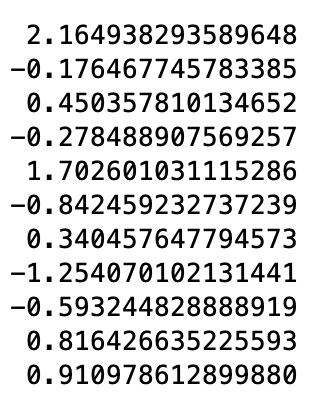
\includegraphics[width=0.4\linewidth]{lateximages/eleven.png}
  \caption{Eleven randomly generated numbers.}
  \label{fig:boat1}
  \end{figure}
  
  \noindent The mean of the list is 0.2946. The standard deviation is 1.057. The standard error on the mean is 0.302. This result makes sense because the mean of 0.2946 is within the uncertainty of of the mean of $\frac{1}{\sqrt{11}}=0.302$. \newline

 \noindent 3. Using Matlab, I created M=2000 lists of N=11 numbers each. After calculating the means for all of 2000 experiments, I generated a histogram plot of the means. On the next page in figure 2 is a histogram of the means for the 2000 experiments. Note that the histogram looks normal, as expected by the Central Limit Theorem.
  
  \begin{figure}[H]
  \centering
  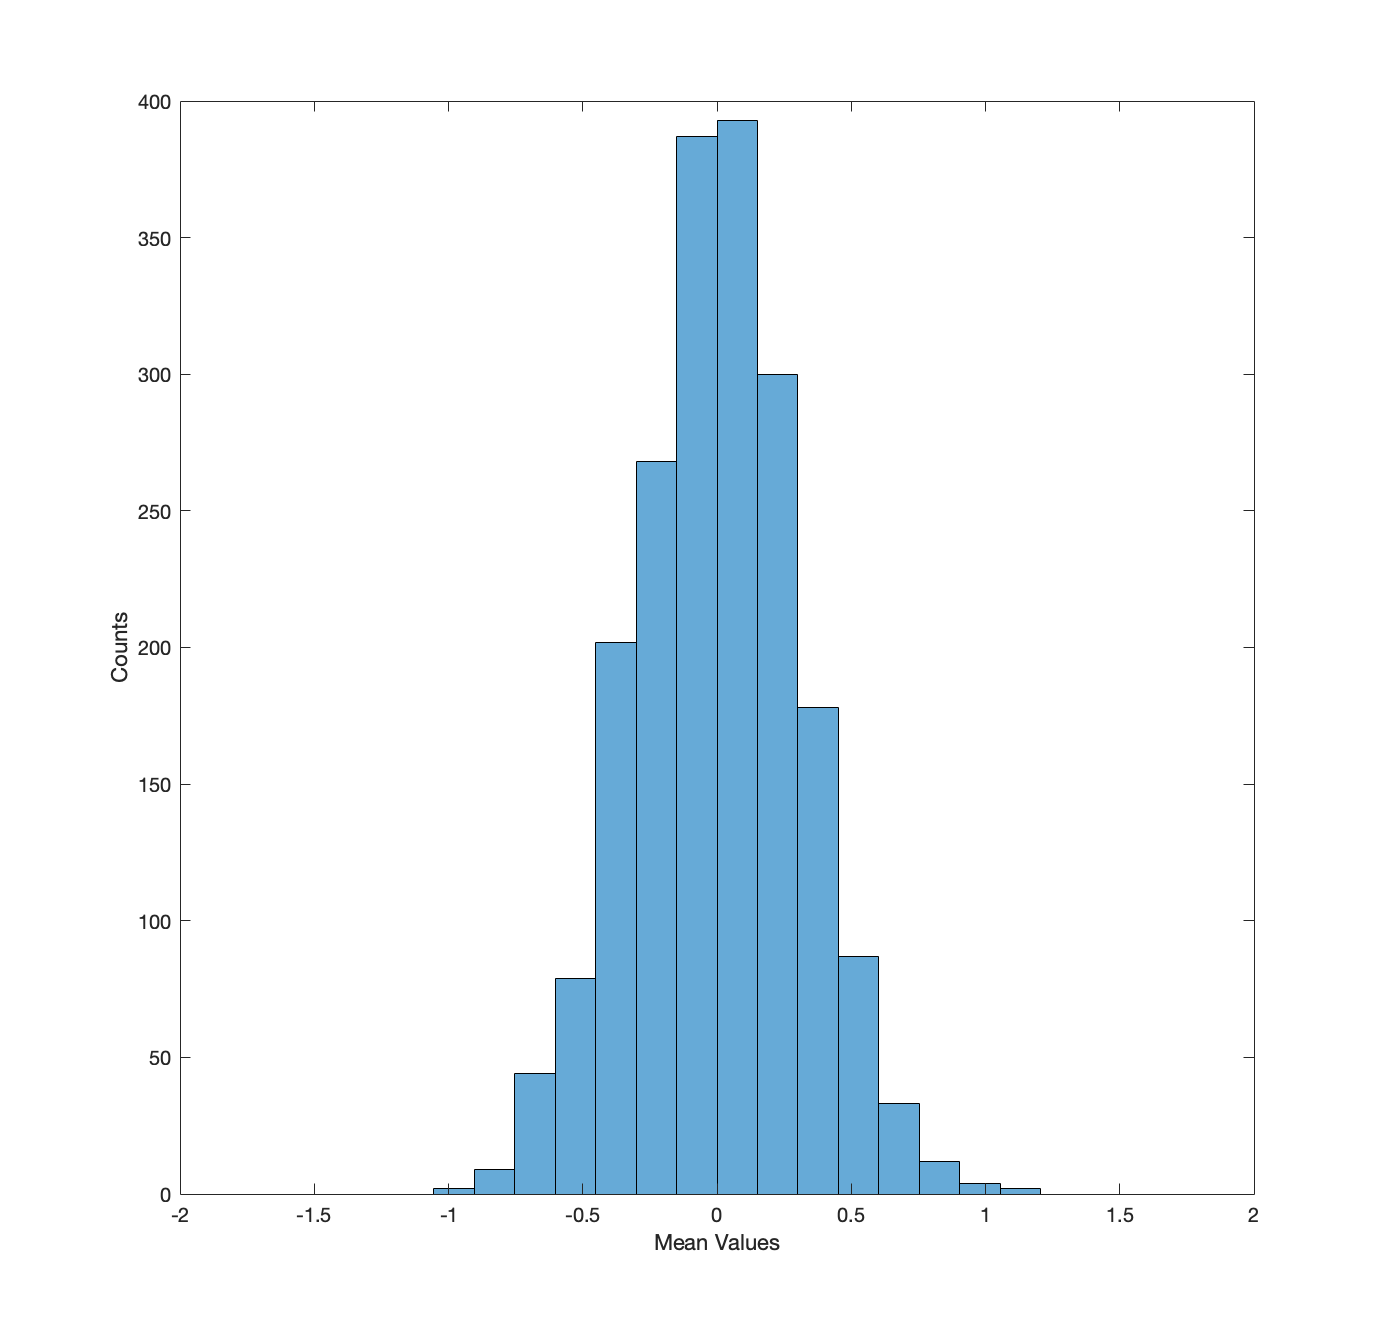
\includegraphics[width=0.8\linewidth]{lateximages/Prob3_3.png}
  \caption{Distribution of means for M=2000 experiments each with N=11 measurements.}
  \label{fig:boat1}
  \end{figure}
  
 Using Matlab’s h.Values function, we find that there are 1348 or 67.4\% of the 2000 experiments within one uncertainty of the mean. And there are 1894 or 94.7\% of the 2000 experiments within 2 uncertainty of the mean. The standard deviation of the means is 0.299, which is comparable to the uncertainty of $\frac{3}{\sqrt{11}}=0.302$.   \newline
 
 
 \noindent 4. We start with a population mean and standard deviation of 0 and 1, respectively.
 
 For \textbf{N=20}, we expect the sample to have:
 
 \[ Mean=0\]
  \[ Standard\hspace{1mm}Deviation=1\]
   \[ Standard\hspace{1mm}Error=\sigma_{\mu}=\frac{\sigma}{\sqrt{N}}=\frac{1}{\sqrt{20}}\] 


Now I generated a list of N=20 random numbers using the randn function and found that it gave:

 \[ Mean=0.283\]
  \[ Standard\hspace{1mm}Deviation=0.882\]
   \[ Standard\hspace{1mm}Error=\sigma_{\mu}=\frac{\sigma}{\sqrt{N}}=\frac{1}{\sqrt{20}}\] 
   
   This result makes sense because the mean of 0.283 is within two uncertainties of the mean of $\frac{1}{\sqrt{20}}=0.223$. Below is a histogram of the means for the 2000 experiments each with N=20 normally distributed numbers.
 
   \begin{figure}[H]
  \centering
  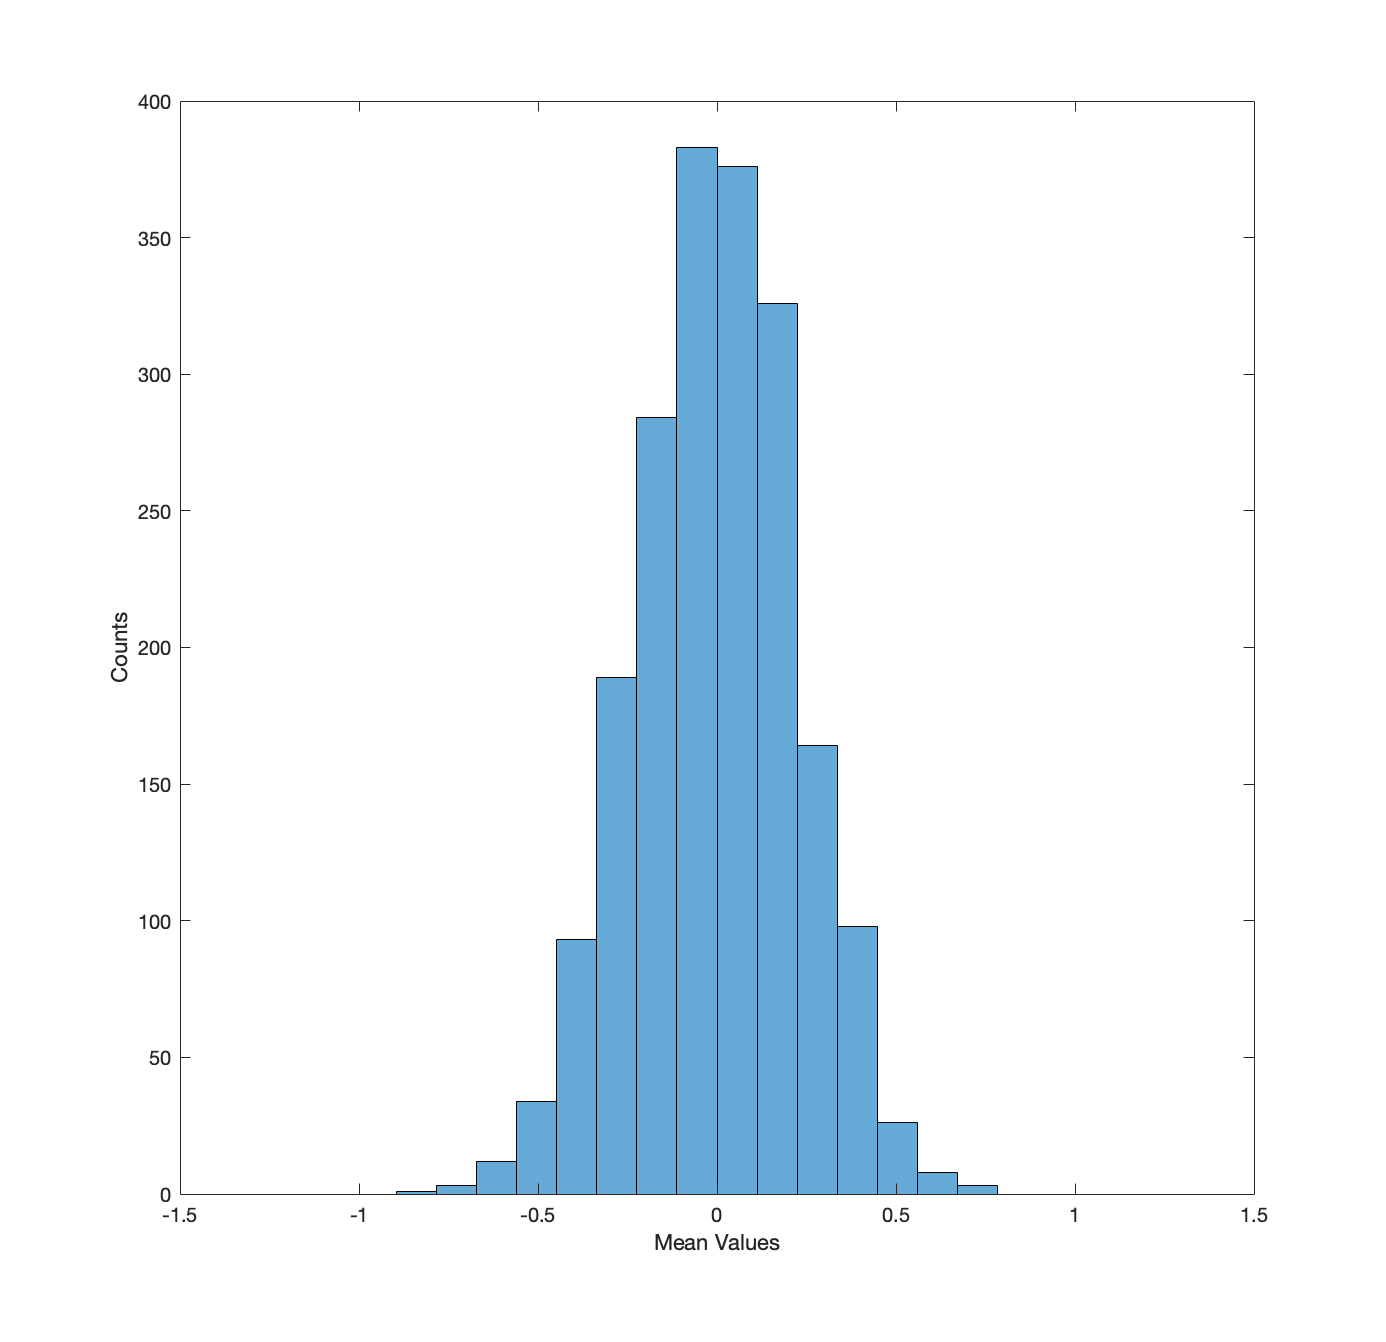
\includegraphics[width=0.8\linewidth]{lateximages/Prob3_4_20.png}
  \caption{Distribution of means for M=2000 experiments each with N=20 measurements.}
  \label{fig:boat1}
  \end{figure}
  
  Using Matlab’s h.Values function, we find that there are 1369 or 68.4\% within one uncertainty of the mean. And there are 1913 or 95.6\% within 2 uncertainty of the mean. The standard deviation of the means is 0.255, which is comparable to the uncertainty of $\frac{1}{\sqrt{20}}=0.223$.  \newline
  
  For \textbf{N=40}, we expect the sample to have:
 
 \[ Mean=0\]
  \[ Standard\hspace{1mm}Deviation=1\]
   \[ Standard\hspace{1mm}Error=\sigma_{\mu}=\frac{\sigma}{\sqrt{N}}=\frac{1}{\sqrt{40}}\] 


Now I generated a list of N=40 random numbers using the randn function and found that it gave:

 \[ Mean=0.024\]
  \[ Standard\hspace{1mm}Deviation=1.07\]
   \[ Standard\hspace{1mm}Error=\sigma_{\mu}=\frac{\sigma}{\sqrt{N}}=\frac{1}{\sqrt{40}}\] 
   
   This result makes sense because the mean of 0.024 is within the uncertainty of of the mean of $\frac{1}{\sqrt{40}}=0.158$. Below is a histogram of the means for the 2000 experiments each with N=40 normally distributed numbers.
 

   \begin{figure}[H]
  \centering
  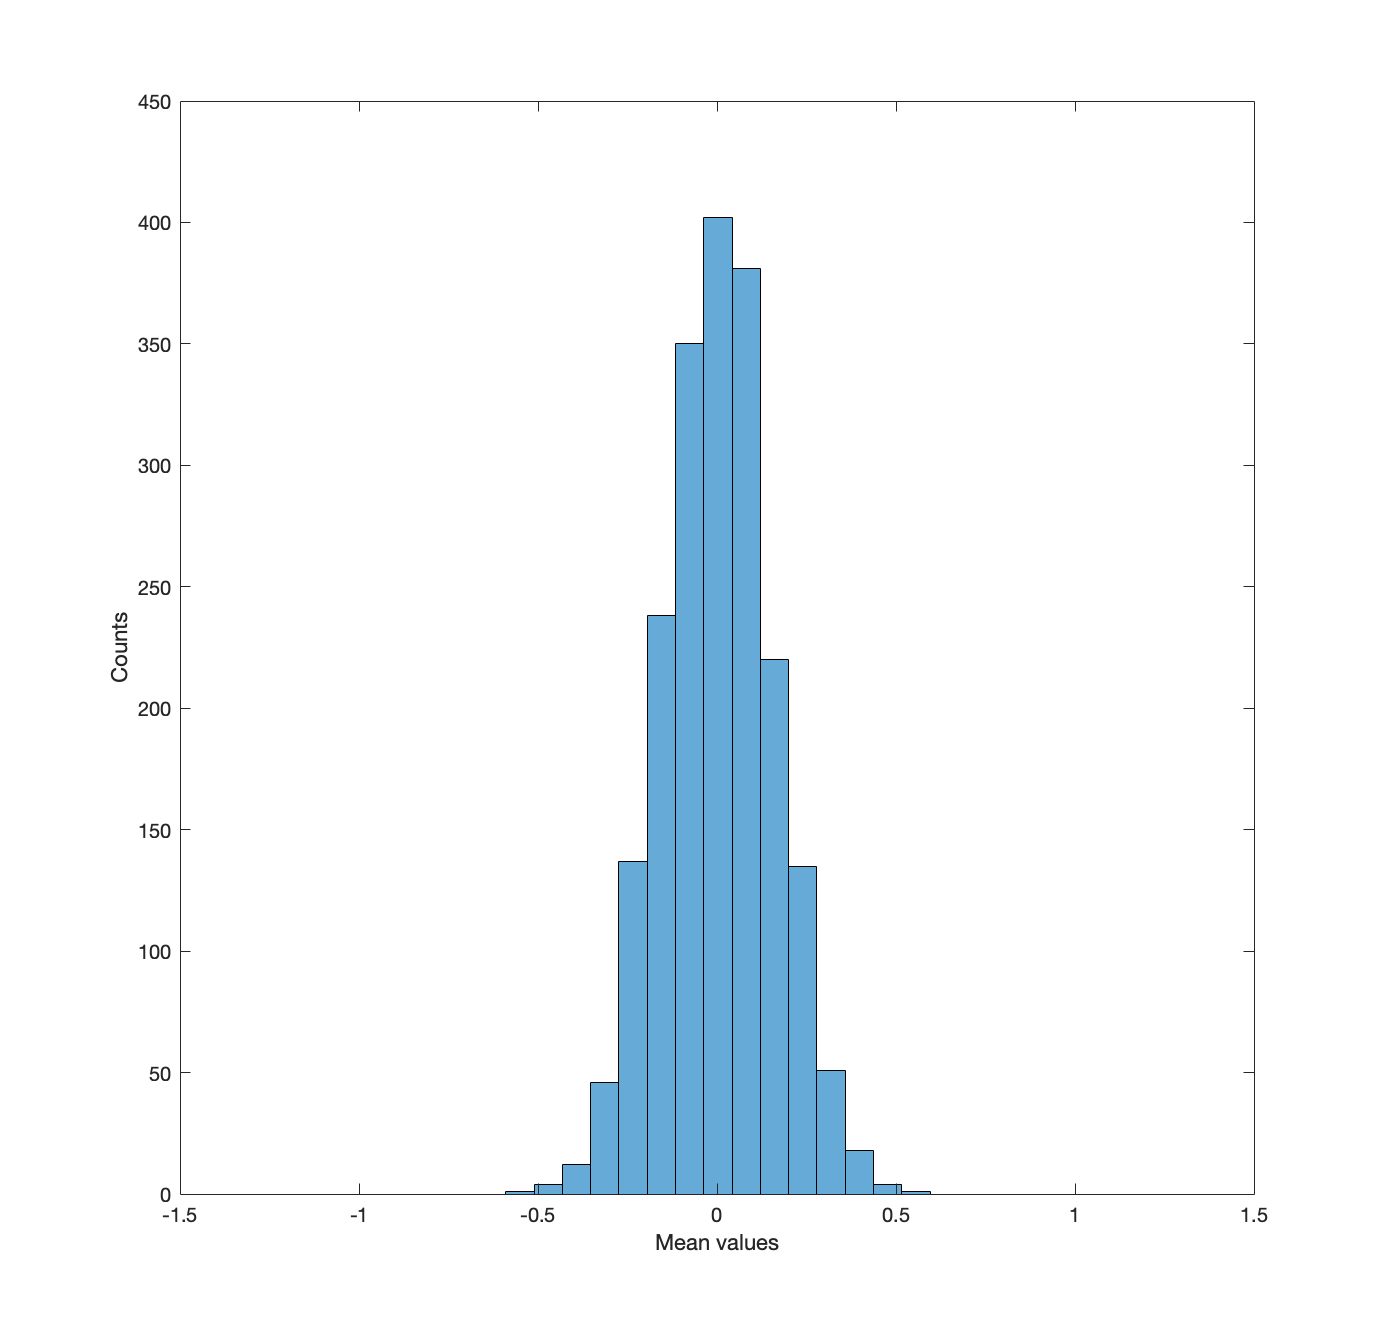
\includegraphics[width=0.8\linewidth]{lateximages/Prob3_4_40.png}
  \caption{Distribution of means for M=2000 experiments each with N=40 measurements.}
  \label{fig:boat1}
  \end{figure}
  
Using Matlab’s h.Values function, we find that there are 1371 or 68.5\% within one uncertainty of the mean. And there are 1909 or 95.5\% within 2 uncertainty of the mean. The standard deviation in the means is 0.154, which is comparable to the uncertainty of $\frac{1}{\sqrt{40}}=0.158$.  \newline
  
  For \textbf{N=80}, we expect the sample to have:
 
 \[ Mean=0\]
  \[ Standard\hspace{1mm}Deviation=1\]
   \[ Standard\hspace{1mm}Error=\sigma_{\mu}=\frac{\sigma}{\sqrt{N}}=\frac{1}{\sqrt{80}}\] 


Now I generated a list of N=80 random numbers using the randn function and found that it gave:

 \[ Mean=0.129\]
  \[ Standard\hspace{1mm}Deviation=1.14\]
   \[ Standard\hspace{1mm}Error=\sigma_{\mu}=\frac{\sigma}{\sqrt{N}}=\frac{1}{\sqrt{80}}\]
   
     This result makes sense because the mean of 0.129 is within two uncertainties of the mean of $\frac{1}{\sqrt{80}}=0.112$. Below is a histogram of the means for the 2000 experiments each with N=80 normally distributed numbers.
 

   \begin{figure}[H]
  \centering
  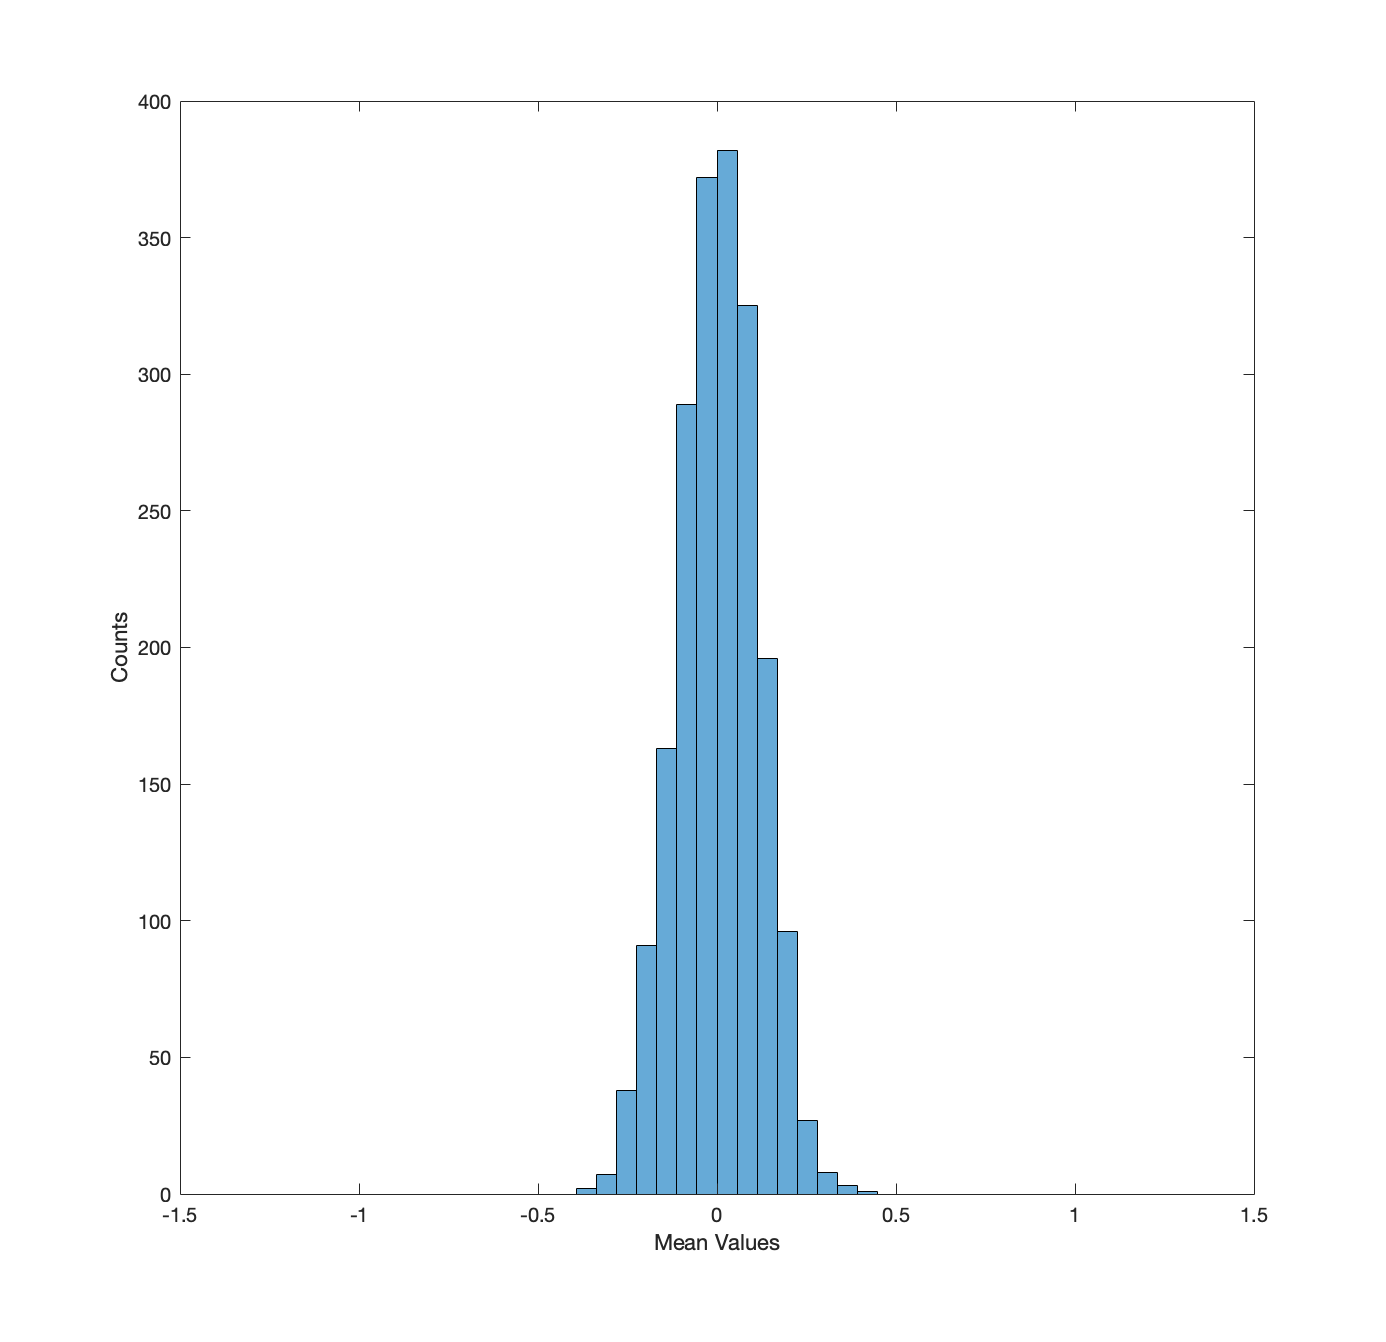
\includegraphics[width=0.8\linewidth]{lateximages/Prob3_4_80.png}
  \caption{Distribution of means for M=2000 experiments each with N=80 measurements.}
  \label{fig:boat1}
  \end{figure}

Using Matlab’s h.Values function, we find that there are 1368  or 68.4\% within one uncertainty of the mean. And there are 1914 or 95.7\% within 2 uncertainty of the mean. The standard deviation in the means is 0.1117, which is comparable to the uncertainty of $\frac{1}{\sqrt{80}}=0.112$.  \newline


For \textbf{N=800}, we expect the sample to have:
 
 \[ Mean=0\]
  \[ Standard\hspace{1mm}Deviation=1\]
   \[ Standard\hspace{1mm}Error=\sigma_{\mu}=\frac{\sigma}{\sqrt{N}}=\frac{1}{\sqrt{800}}\] 


Now I generated a list of N=800 random numbers using the randn function and found that it gave:

 \[ Mean=0.005\]
  \[ Standard\hspace{1mm}Deviation=1.005\]
   \[ Standard\hspace{1mm}Error=\sigma_{\mu}=\frac{\sigma}{\sqrt{N}}=\frac{1}{\sqrt{800}}\] 
   
   This result makes sense because the mean of 0.005 is within the uncertainty of the mean of $\frac{1}{\sqrt{800}}=0.035$. Below is a histogram of the means for the 2000 experiments each with N=800 normally distributed numbers.
 

 \begin{figure}[H]
  \centering
  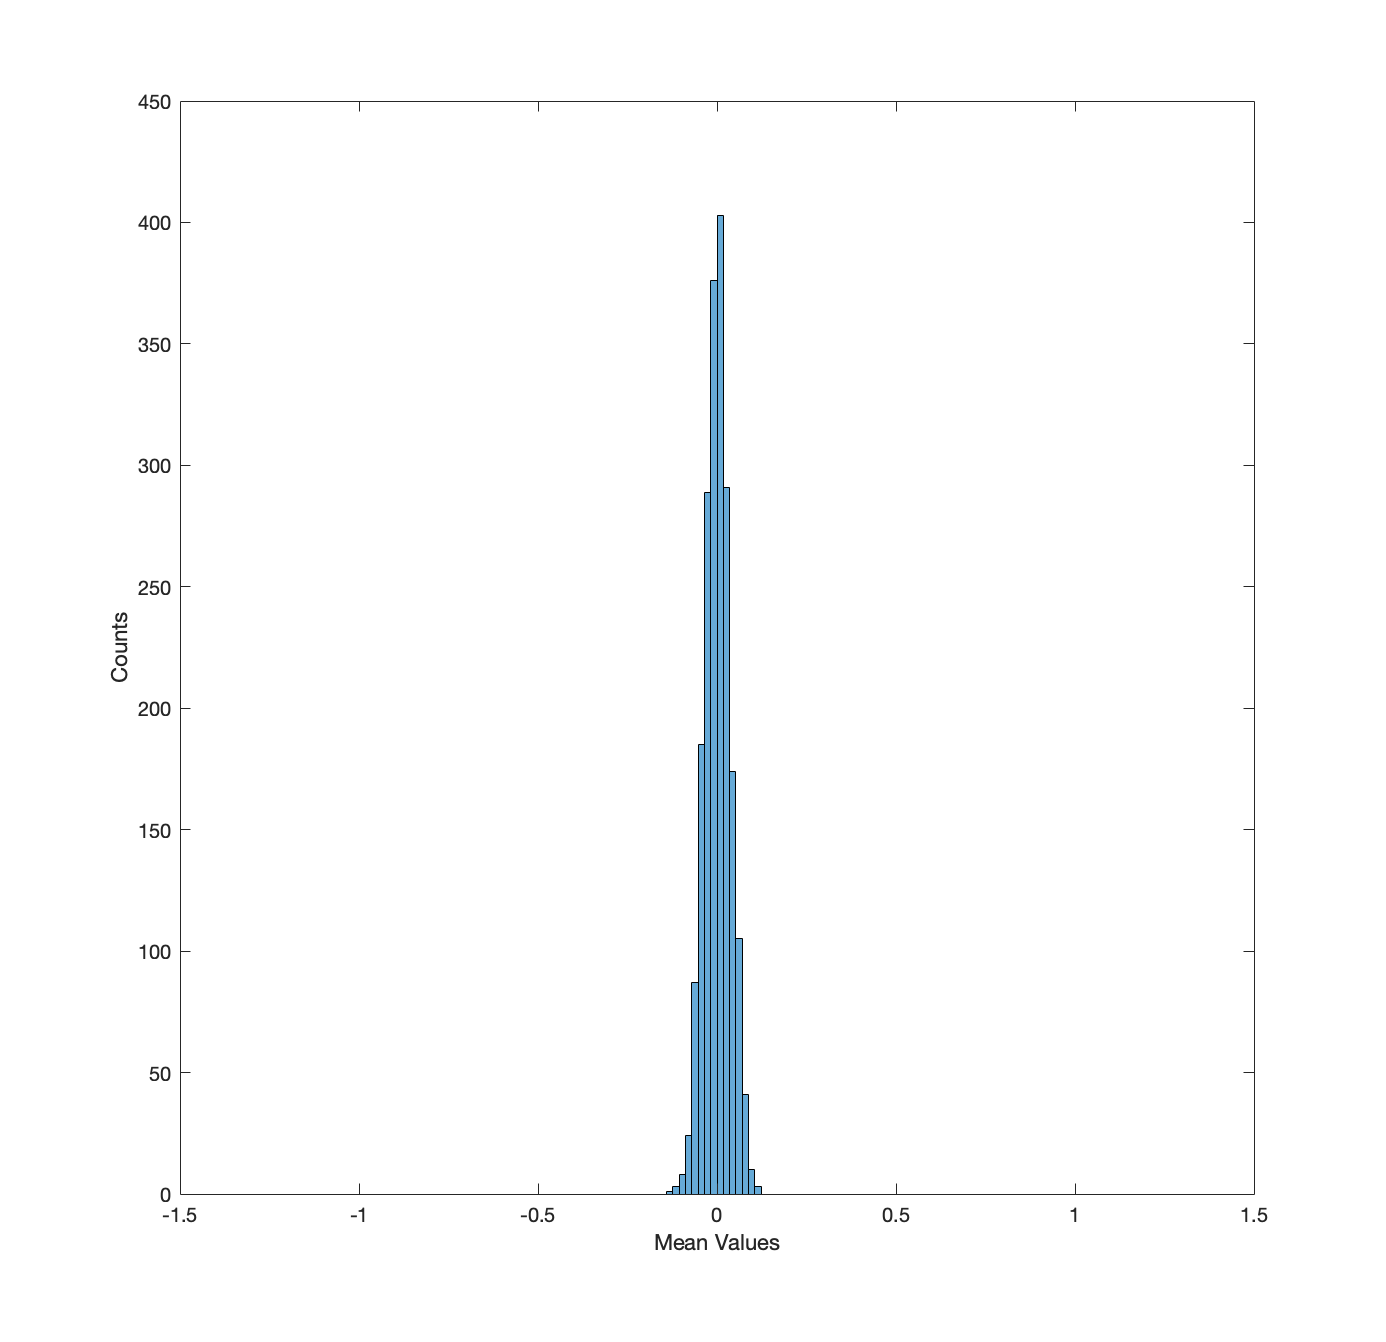
\includegraphics[width=0.8\linewidth]{lateximages/Prob3_4_800.png}
  \caption{Distribution of means for M=2000 experiments each with N=800 measurements.}
  \label{fig:boat1}
  \end{figure}
  
  Using Matlab’s h.Values function, we find that there are 1359 or 67.9\% within one uncertainty of the mean. And there are 1910 or 95.5\% within 2 uncertainty of the mean. The standard deviation in the means is 0.03548, which is comparable to the uncertainty of $\frac{1}{\sqrt{800}}=0.035$. 
  
\section*{Problem 4}
1. The mean of an exponential distribution $e^{-x}dx$ should be:
\[ \mu=\int_{0}^{\infty} xe^{-x} dx=\lim_{n\to \infty}[-xe^{-x}-e^{-x}]^n_0=1\] 

\noindent The standard deviation of an exponential distribution should be 
\[ \sigma=\sqrt{\int_{0}^{\infty} (x-\mu)^2e^{-x} dx}=\sqrt{\int_{0}^{\infty} (x-1)^2e^{-x} dx}=1\] 

\noindent or more generally for a distribution of the form $P(x)=\lambda e^{-x}$, the mean is $\lambda$ and the standard deviation is also $\lambda$. The error on the mean for an experiment with N=300 random samples should be:

\[ Standard\hspace{1mm}Error=\sigma_{\mu}=\frac{\sigma}{\sqrt{N}}=\frac{1}{\sqrt{300}}\hspace{1mm}or\hspace{1mm}\frac{\lambda}{\sqrt{300}}\hspace{1mm}for\hspace{1mm}P(x)=\lambda e^{-x} \] 

By the central limit theorem, when a growing number of random samples are taken from the parent population, the sampling distribution of the means of the random samples will become approximately normally distributed with mean $\mu$ and standard deviation $\frac{\sigma}{\sqrt{ N}}$ as the sample size N becomes larger, regardless of the shape of the parent distribution. Given this, I expect that the distribution of means for M=600 experiments should look approximately normal with the uncertainty of the means for a parent population mean of 1 to be $\frac{1}{\sqrt{300}}$.  \\


\noindent 2. Using matlab's exprnd function, I generated a list of 300 exponentially distributed random numbers with true mean 1. The mean of the list was $\mu=1.018$ and the standard deviation was $\sigma=1.0080$. This is expected since an exponential distribution should have the same value for the mean and standard deviation, and the mean of 1.018 is within the uncertainty of the mean of $\frac{1}{\sqrt{300}}=0.057$  \newline

\noindent 3.     Using Matlab, I created M=600 lists of N=300 numbers each. After calculating the means for all of 600 experiments, I generated a histogram plot of the means. On the beginning of the next page is a histogram of the distribution of means for M=600 Lists of N=300 exponentially distributed numbers. Note that the histogram looks normal, as expected by the Central Limit Theorem.

 \begin{figure}[H]
  \centering
  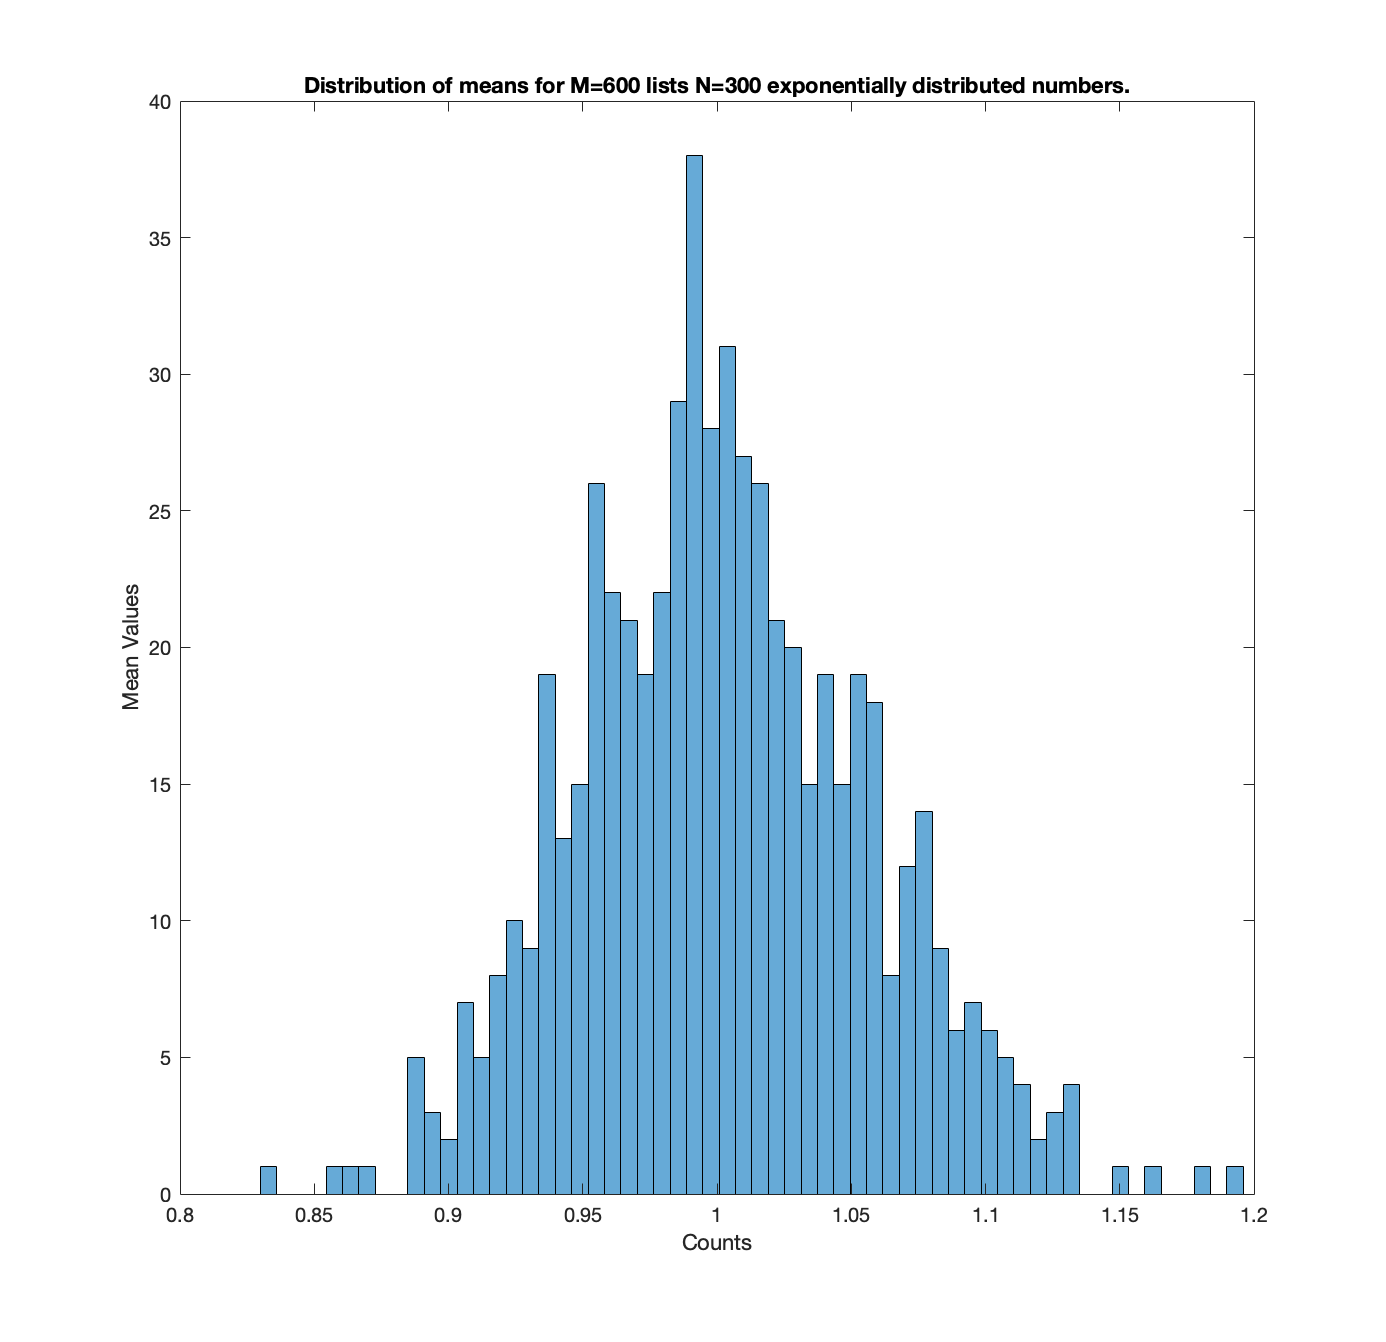
\includegraphics[width=0.8\linewidth]{lateximages/Prob4_3.png}
  \caption{Distribution of means for M=600 lists of N=300 exponentially distributed numbers.}
  \label{fig:boat2}
  \end{figure}  
  
    The standard deviation of the means is 0.054, which is less than the uncertainty of $\frac{1}{\sqrt{300}}=0.057$. \newline
  
\noindent 4.   For \textbf{N=3000}, we expect the sample to have:
 
 \[ Mean=1\]
  \[ Standard\hspace{1mm}Deviation=1\]
   \[ Standard\hspace{1mm}Error=\sigma_{\mu}=\frac{1}{\sqrt{3000}}\] 


Now I generated a list of N=3000 exponentially distributed random numbers using the exprnd function and found that it gave:

 \[ Mean=1.004\]
  \[ Standard\hspace{1mm}Deviation=0.9806\]
   \[ Standard\hspace{1mm}Error=\sigma_{\mu}=\frac{1}{\sqrt{3000}}\] 
   
   This is expected since an exponential distribution should have the same value for the mean and standard deviation, and the mean of 1.0004 is within the uncertainty of the mean of $\frac{1}{\sqrt{3000}}=0.018$.
   
   Below is a histogram of the distribution of means for M=600 Lists of N=3000 exponentially distributed numbers. Note that the histogram looks normal, as expected by the Central Limit Theorem.
   
    \begin{figure}[H]
  \centering
  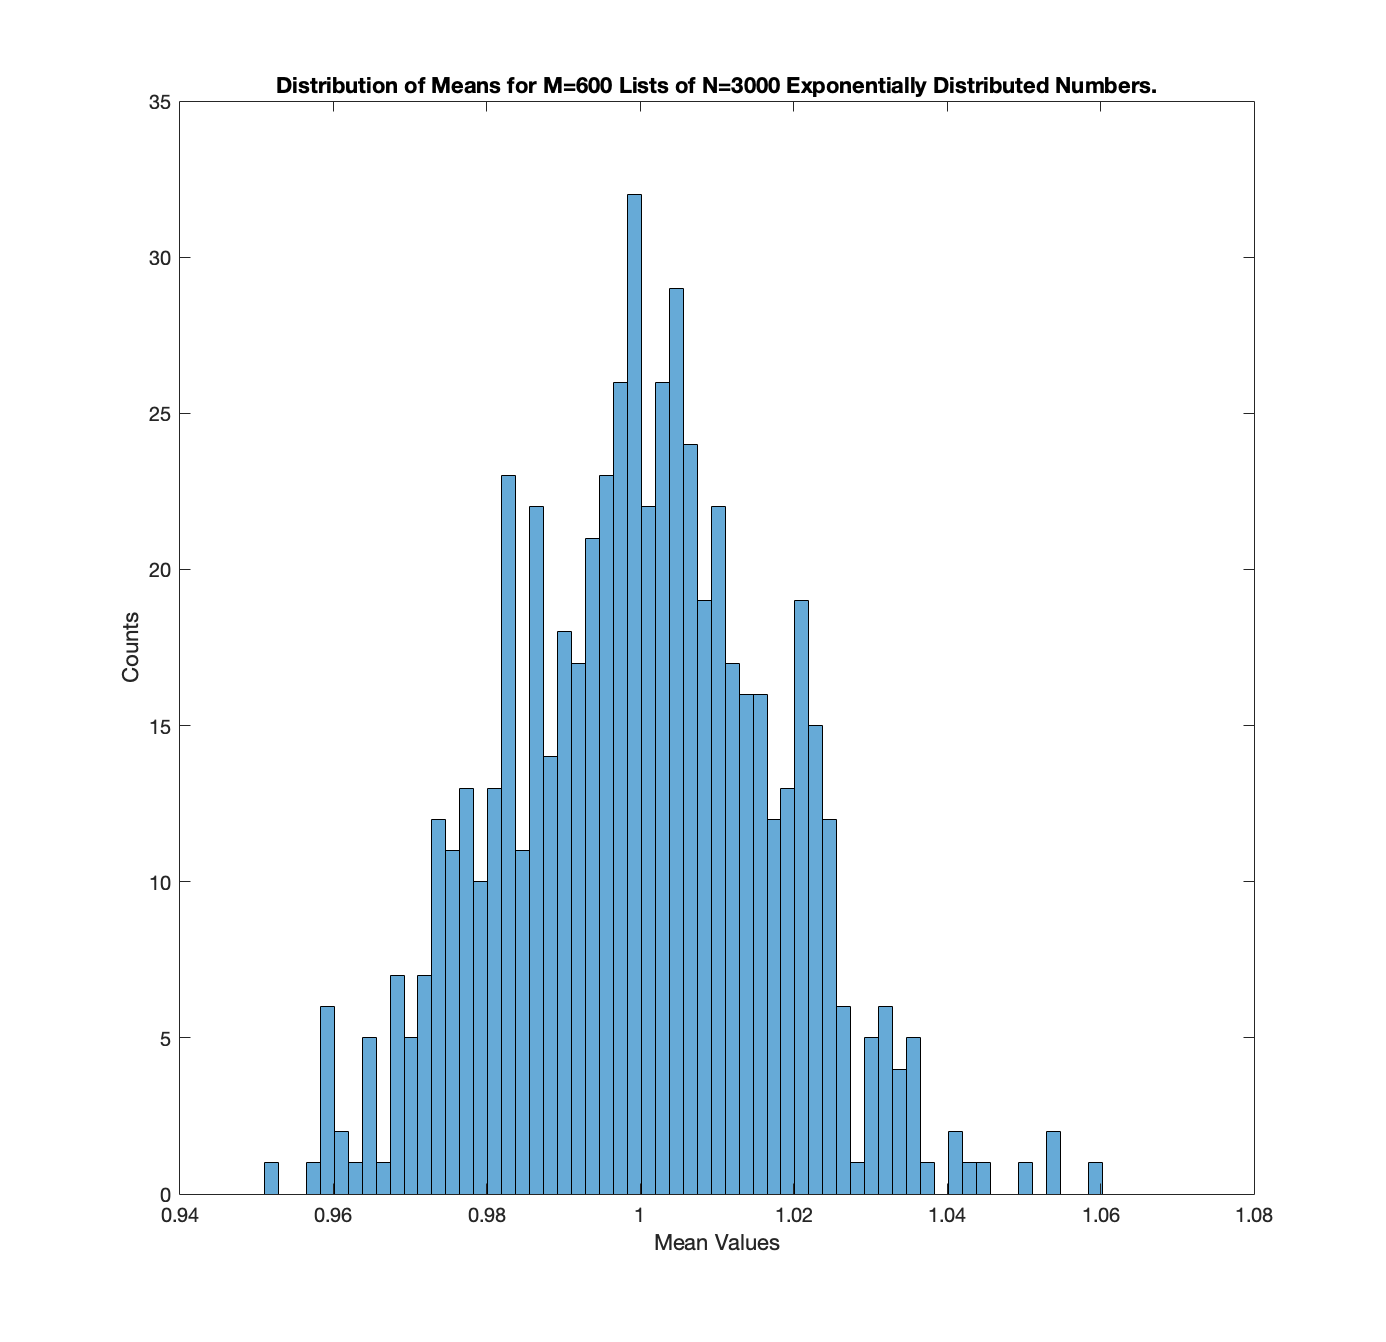
\includegraphics[width=0.8\linewidth]{lateximages/Prob4_4_3000.png}
  \caption{Distribution of Means for M=600 Lists of N=3000 Exponentially Distributed Numbers.}
  \label{fig:boat1}
  \end{figure}
  
  The standard deviation of the means is 0.0177, which is comparable to the uncertainty of $\frac{1}{\sqrt{3000}}=0.018$. \newline
  
  For \textbf{N=60000}, we expect the sample to have:
 
 \[ Mean=1\]
  \[ Standard\hspace{1mm}Deviation=1\]
   \[ Standard\hspace{1mm}Error=\sigma_{\mu}=\frac{1}{\sqrt{60000}}\] 

  
  Now I generated a list of N=60000 exponentially distributed random numbers using the exprnd function and found that it gave:

 \[ Mean=0.998\]
  \[ Standard\hspace{1mm}Deviation=0.991\]
   \[ Standard\hspace{1mm}Error=\sigma_{\mu}=\frac{1}{\sqrt{60000}}\] 
   
    This is expected since an exponential distribution should have the same value for the mean and standard deviation, and the mean of 0.998 is within the uncertainty of the mean of $\frac{1}{\sqrt{60000}}=0.0041$.
   
   Below is a histogram of the distribution of means for M=600 Lists of N=60000 exponentially distributed numbers. Note that the histogram looks normal, as expected by the Central Limit Theorem.
   
    \begin{figure}[H]
  \centering
  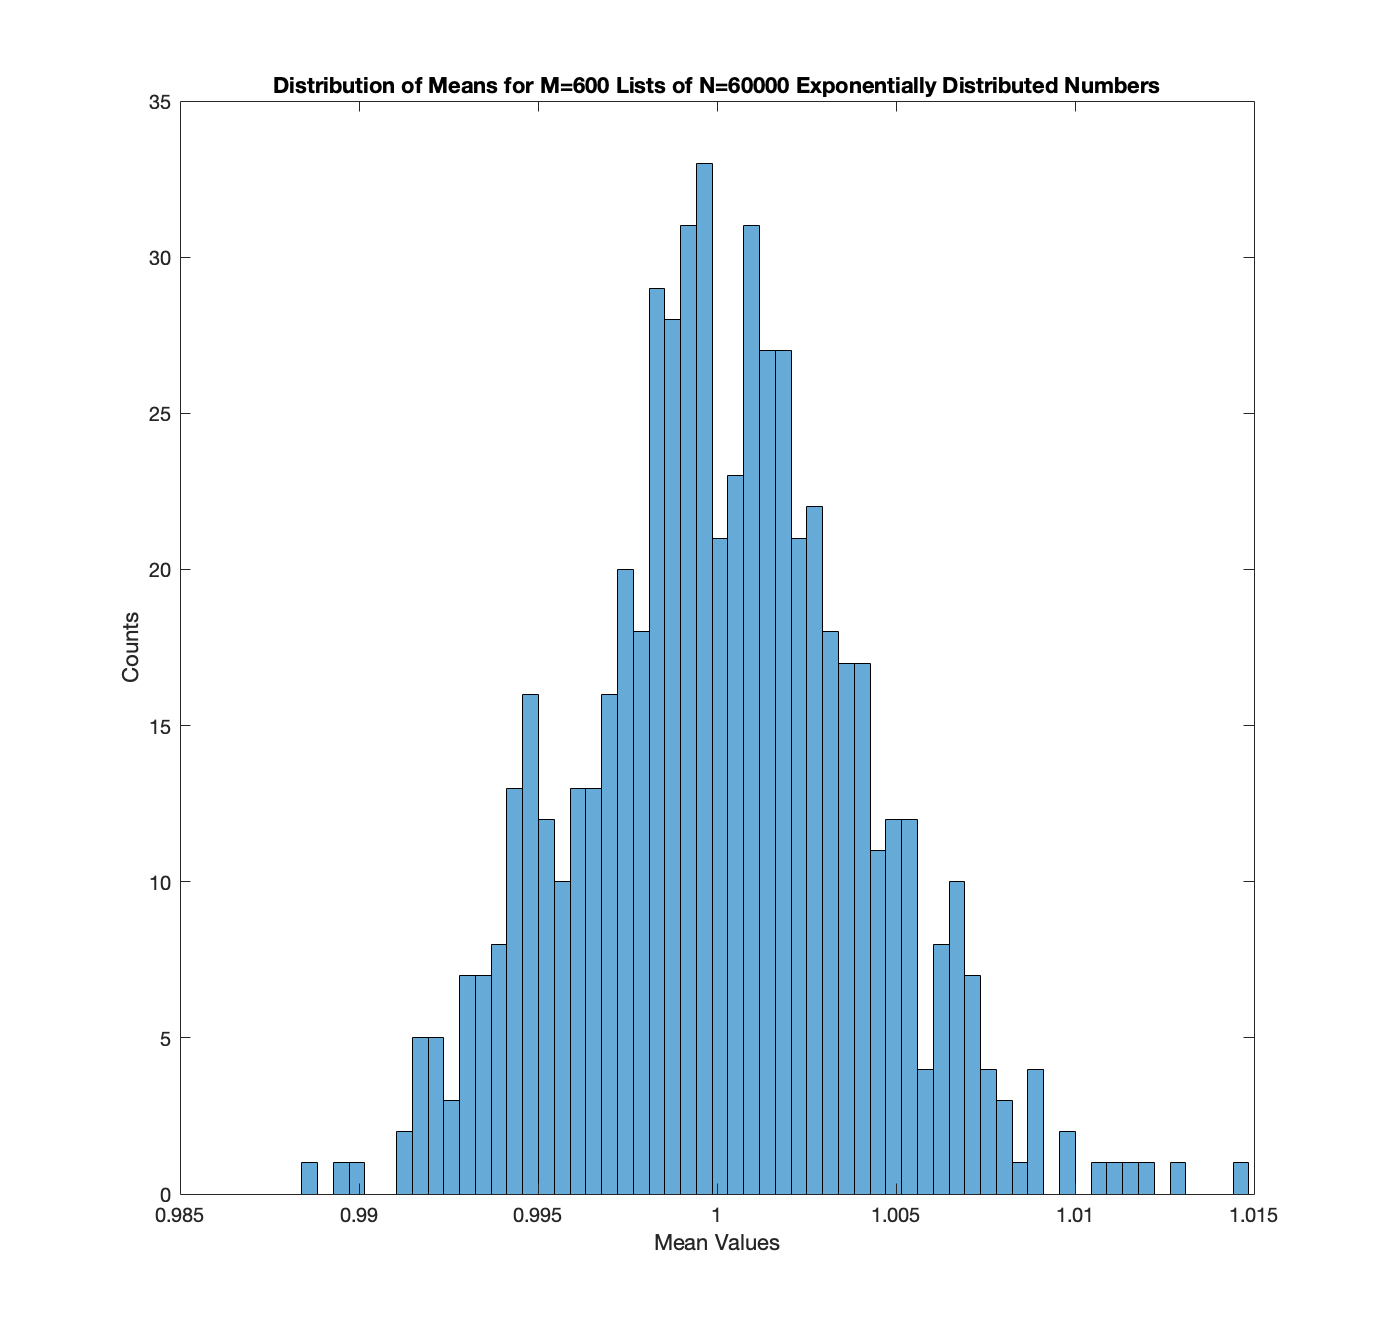
\includegraphics[width=0.8\linewidth]{lateximages/Prob4_4_60000.png}
  \caption{Distribution of Means for M=600 Lists of N=60000 Exponentially Distributed Numbers.}
  \label{fig:boat1}
  \end{figure}
  
  The standard deviation of the means is 0.004, which is comparable to the uncertainty of $\frac{1}{\sqrt{60000}}=0.0041$. 

\section*{Problem 5} 
1. Using matlab's histogram function, I plotted the peak dataset from the gamma-ray experiment of 1000 hits. On the next page in figure 10 is the histogram of the distribution of energies using 50 bins with error bars for each bin.
   \begin{figure}[H]
  \centering
  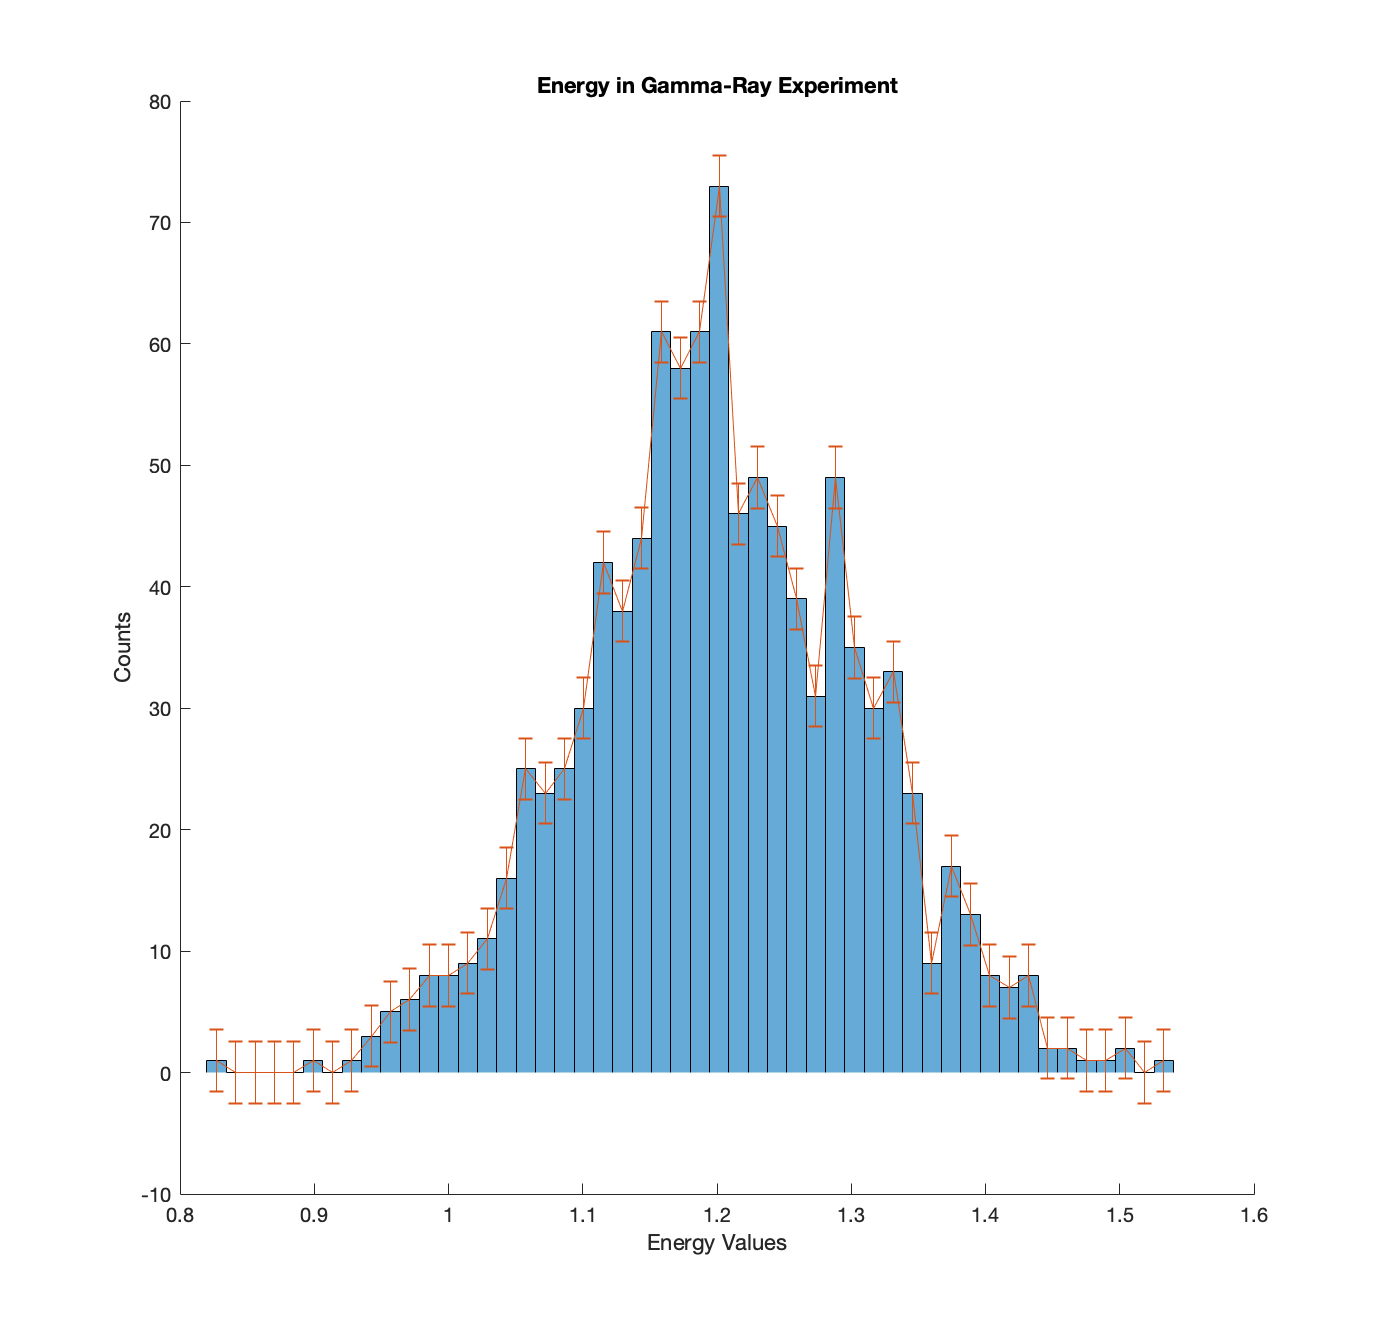
\includegraphics[width=0.8\linewidth]{lateximages/Prob5_1.png}
  \caption{Histogram of the Distribution of Energies in Gamma-Ray experiment.}
  \label{fig:boat2}
  \end{figure}  
  
 
\noindent  2. Using Matlab, we find that the mean of the data is 1.2027 and the standard deviation is 0.1038.
\\ \\
\noindent 3. Now using Matlab's fitting functions and the GaussianFit function from the Physics 111B lab website, I fitted the data to a Gaussian function. The fitted data can be found on figure 12 for Problem 3.4. On the next page in figure 11 is a histogram of the energies with the Gaussian fit overlayed.

\begin{figure}[H]
  \centering
  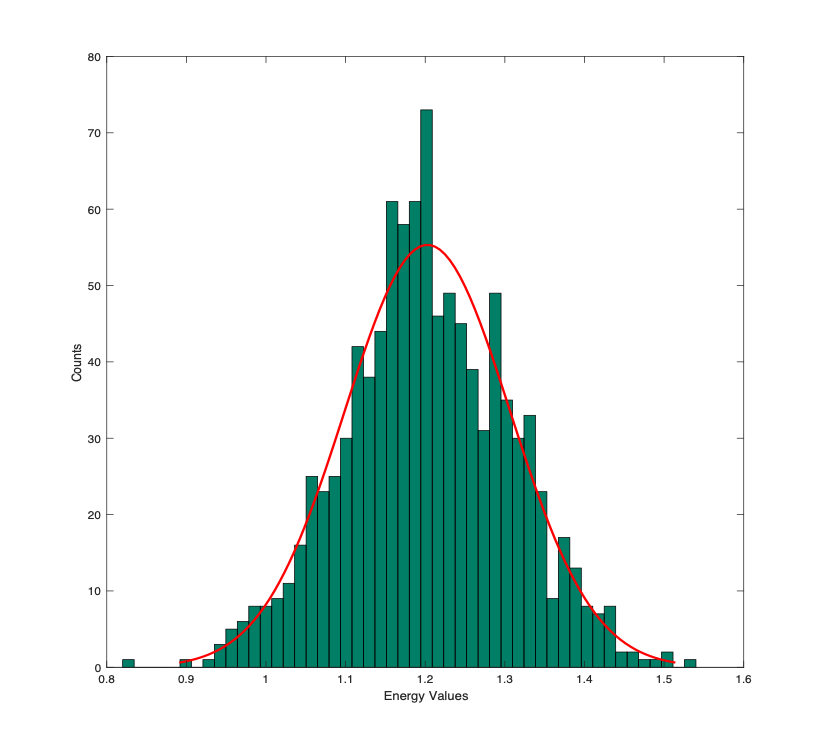
\includegraphics[width=0.8\linewidth]{lateximages/Prob5_3.png}
  \caption{Histogram of the Distribution of Energies in Gamma-Ray experiment with Gaussian Fit.}
  \label{fig:boat2}
  \end{figure}
  
  The fitted curve gives a mean of 1.201 and a standard deviation of 0.102 whereas the actual data gives $\mu=1.2027$ and $\sigma=0.1038$, so the values of the fitted curve are very close to the actual data's mean and standard deviation.  \newline
  
\noindent 4. Using the GaussianFit program from the Physics 111b website, the Gaussian fit provides an amplitude A=55.934, $\mu=1.201$, and $\sigma=0.102$. The GaussianFit function also allows us to get a reduced chi-squared value ($\frac{\chi^2}{df}$). The unreduced chi-squared value gives us $\chi^2=47$ (50 bins minus 3 fitted parameters), which makes sense because that is the number of degrees of freedom we have, and the reduced chi-squared gives us the value $\frac{\chi^2}{df}=1$, meaning the Gaussian fit is a very good fit to the data. The figure 12 on the next page shows the results of our fit, including the reduced chi-squared value (chi2red). 

\begin{figure}[H]
  \centering
  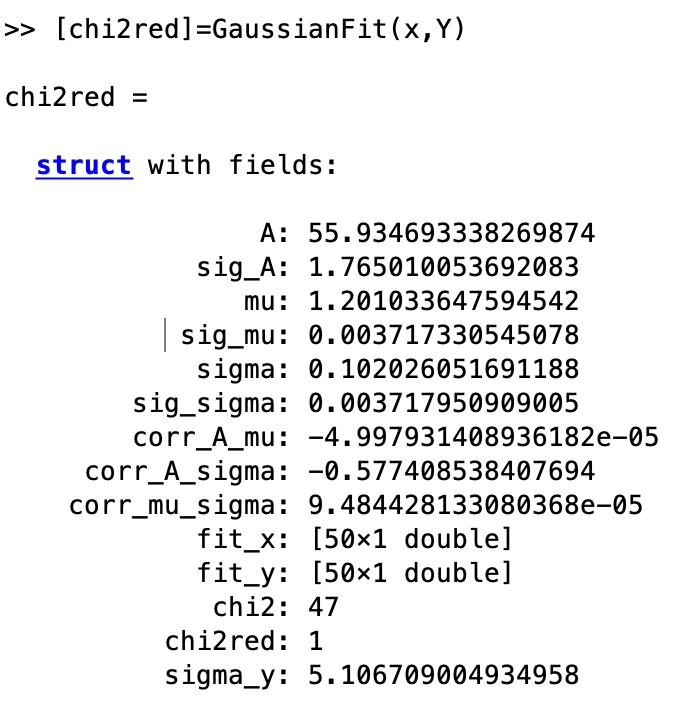
\includegraphics[width=0.5\linewidth]{lateximages/Prob5_4.png}
  \caption{Fitted Parameters for the Gaussian fit of the Energies using the GaussianFit function.}
  \label{fig:boat2}
  \end{figure}

\section*{Problem 6} 
1. The least square method for a straight line (y=A+Bx) with equal weights uses the following equations:
\[ A=\frac{\Sigma x^2\Sigma y-\Sigma x\Sigma xy}{\Delta}\hspace{1mm}and\hspace{1mm}B=\frac{N\Sigma xy-\Sigma x\Sigma y}{\Delta} \]
\noindent where N is the number of pairs of points and $\Delta=N\Sigma x^2-(\Sigma x)^2$. So for A and B, we get:

\[ intercept=A=\frac{\Sigma x^2\Sigma y-\Sigma x\Sigma xy}{\Delta}=\frac{20.24*40.50-13.2*61.97}{12*20.24-13.2^2 }=\boxed{0.025}\]

\[ slope=B=\frac{N\Sigma xy-\Sigma x\Sigma y}{\Delta}=\frac{12*61.97-13.2*40.5}{12*20.24-13.2^2}=\boxed{3.045}\]

On the next page in figure 13 is a graph of the data points with the best fit line using the least-squares method.

\begin{figure}[H]
  \centering
  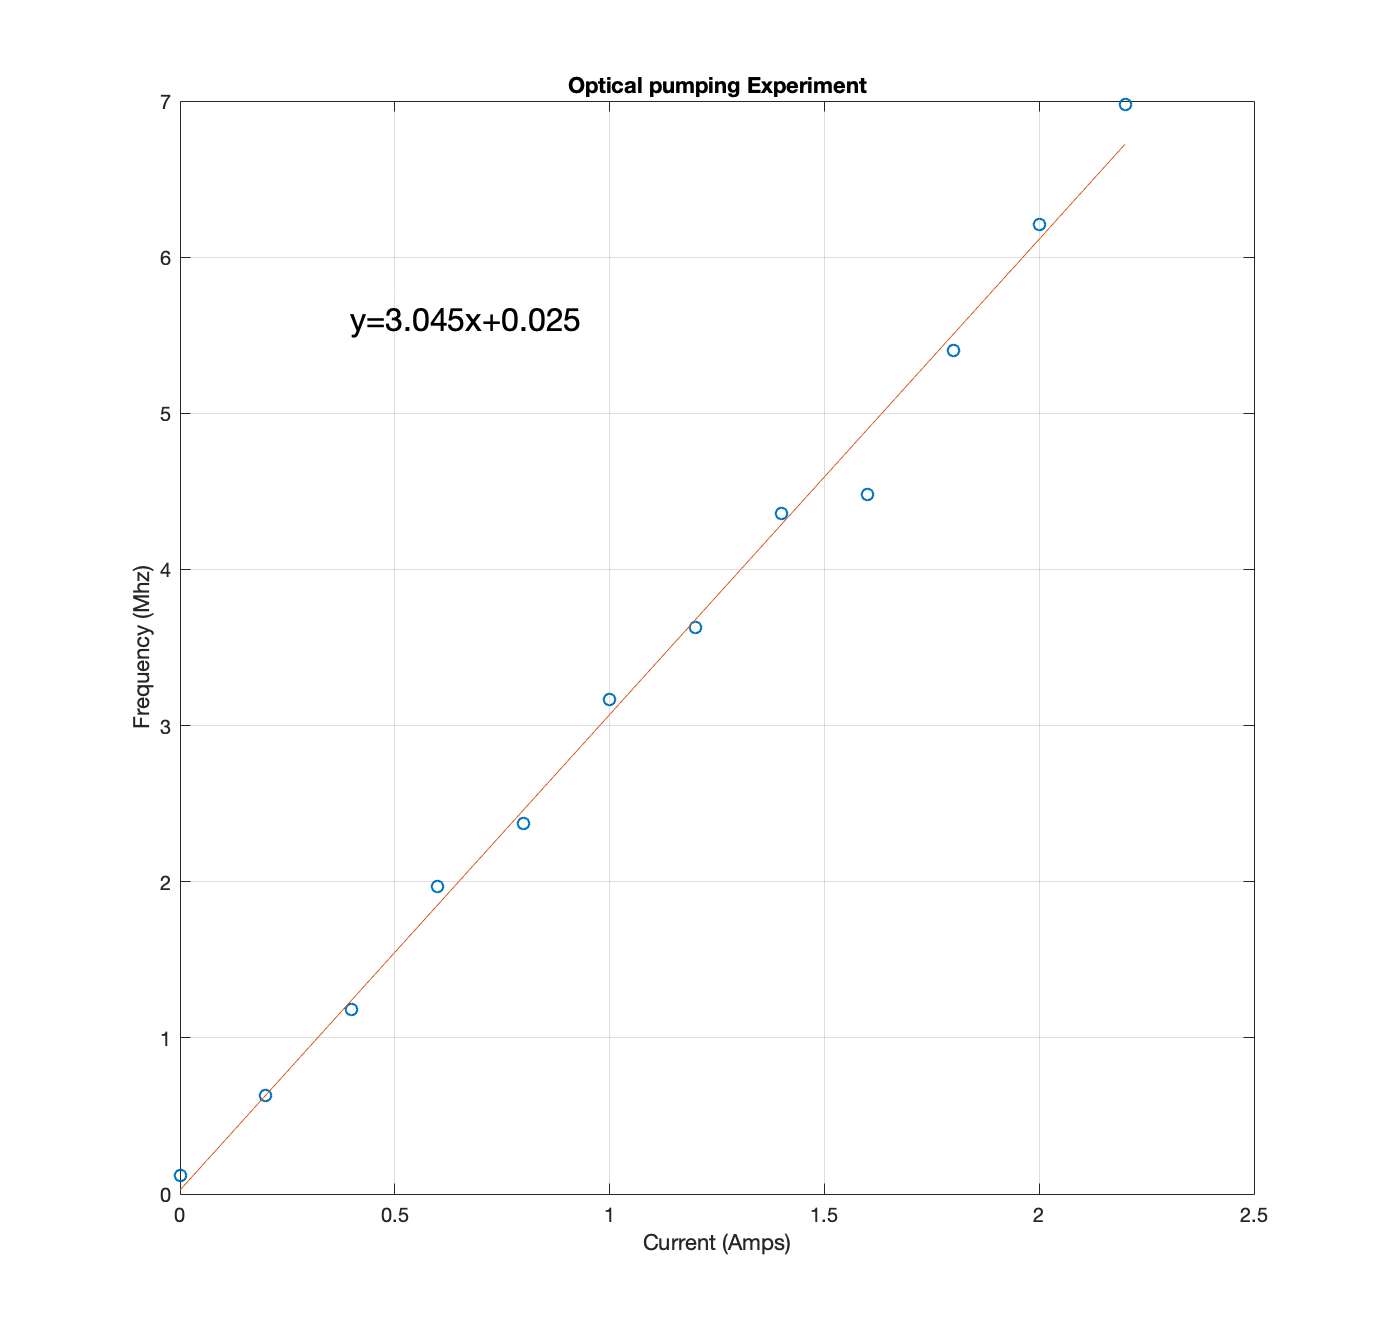
\includegraphics[width=0.8\linewidth]{lateximages/Prob6_1.png}
  \caption{Optical Pumping Experiment with Unweighted least-Squares Fit.}
  \label{fig:boat2}
  \end{figure}  
  
 \noindent 2. The reduced chi-squared value for a linear fit is defined as \[\chi_{\nu}^2=\frac{1}{\nu}\Sigma \frac{(y_i-(mx_i+b))^2}{\sigma_{i}^2}\]
 
 If we assume the uncertainty in the measurement of f to be $\sigma_f=0.024\hspace{0.5mm}Mhz$, we find that reduced chi-squared value is 54.25. This suggests that much of the fit is not within the error bars corresponding to the data. Looking at the table C.4 in Bevington, since we have 10 degrees of freedom (12 data points minus 2 fit parameters), the probability $P_{\chi}(\chi,\nu)$ is much less than 50 percent.
 
If we assume the uncertainty in the measurement of f to be $\sigma_f=0.16\hspace{0.5mm}Mhz$, we find that reduced chi-squared value is 1.22. This suggests that the fit is a reasonably good fit to the data. Looking at the table C.4 in Bevington, the probability $P_{\chi}(\chi,\nu)$ is less than 50 percent. 

However, since both probabilities are much less than 50 percent, it could suggest a better fit to the data is needed. \newline
 
  
\noindent 3. The variance in the frequency can be written as \[\sigma_{y}^2=\frac{1}{N-2}\Sigma{(y_i-(mx_i+b))^2}\] where N is the \# of data points and 2 comes from the \# of fit parameters (in this case the slope and intercept means 2 fit parameters). In our case, using the m and b from part 1, the square root of this gives the uncertainty in y, which turned out to be around \boxed{0.177 Mhz}.
Now the variance in the slope and the intercept can both be found using the propagation of error rules.
The variance in the slope is now \[\sigma_{m}^2=\frac{\sigma_{y}^2}{\Sigma (x_i-\mu_x)^2}\] where $\mu_x$ is the mean of our $x_i$ (current) values. So the uncertainty in our slope is \[slope\hspace{1mm}uncertainty=\sigma_{m}=\sqrt{\frac{\sigma_{y}^2}{\Sigma (x_i-\mu_x)^2}}=\sqrt{\frac{0.177^2}{\Sigma (x_i-1.1)^2}}=\sqrt{\frac{0.177^2}{20.24}}=\boxed{0.039\hspace{0.5mm}Mhz}\]

Now the variance in the intercept is \[\sigma_{b}^2=\sigma_{y}^2*(\frac{1}{N}+\frac{\mu_{x}^2}{\Sigma (x_i-\mu_x)^2})\] 

So the uncertainty in the intercept is \[intercept\hspace{1mm}uncertainty=\sigma_{b}=\sqrt{\sigma_{y}^2*(\frac{1}{N}+\frac{\mu_{x}^2}{\Sigma (x_i-\mu_x)^2})}=\sqrt{0.177^2*(\frac{1}{12}+\frac{1.1^2}{20.24})}=\boxed{0.067\hspace{0.5mm}Mhz}\] 

\noindent 4. The weighted least squares method for a linear fit (y=A+Bx) gives the following equations:
 \[ A=\frac{\Sigma wx^2\Sigma wy-\Sigma wx\Sigma wxy}{\Delta}\hspace{1mm}and\hspace{1mm}B=\frac{\Sigma w\Sigma wxy-\Sigma wx\Sigma wy}{\Delta} \]
 
 \noindent where $\Delta=\Sigma w\Sigma wx^2-(\Sigma wx)^2$, $w_f=\frac{1}{\sigma_f^2}$, and $\sigma_f=0.06+0.05*f(Mhz)$. So for A and B, we get:
 
 \[ intercept=A=\frac{\Sigma wx^2\Sigma wy-\Sigma wx\Sigma wxy}{\Delta}=\frac{241.05*716.07-224.85*735.41}{576.69*241.05-224.85^2 }=\boxed{0.082}\]

\[ slope=B=\frac{\Sigma w\Sigma wxy-\Sigma wx\Sigma wy}{\Delta}=\frac{576.69*735.41-224.85*716.07}{576.69*241.05-224.85^2}=\boxed{2.97}\]

So the slope and intercept of the best-fit line using the weighted least-squares method are 2.97 and 0.082, respectively. Here’s the following graph on the next page in figure 14:

\begin{figure}[H]
  \centering
  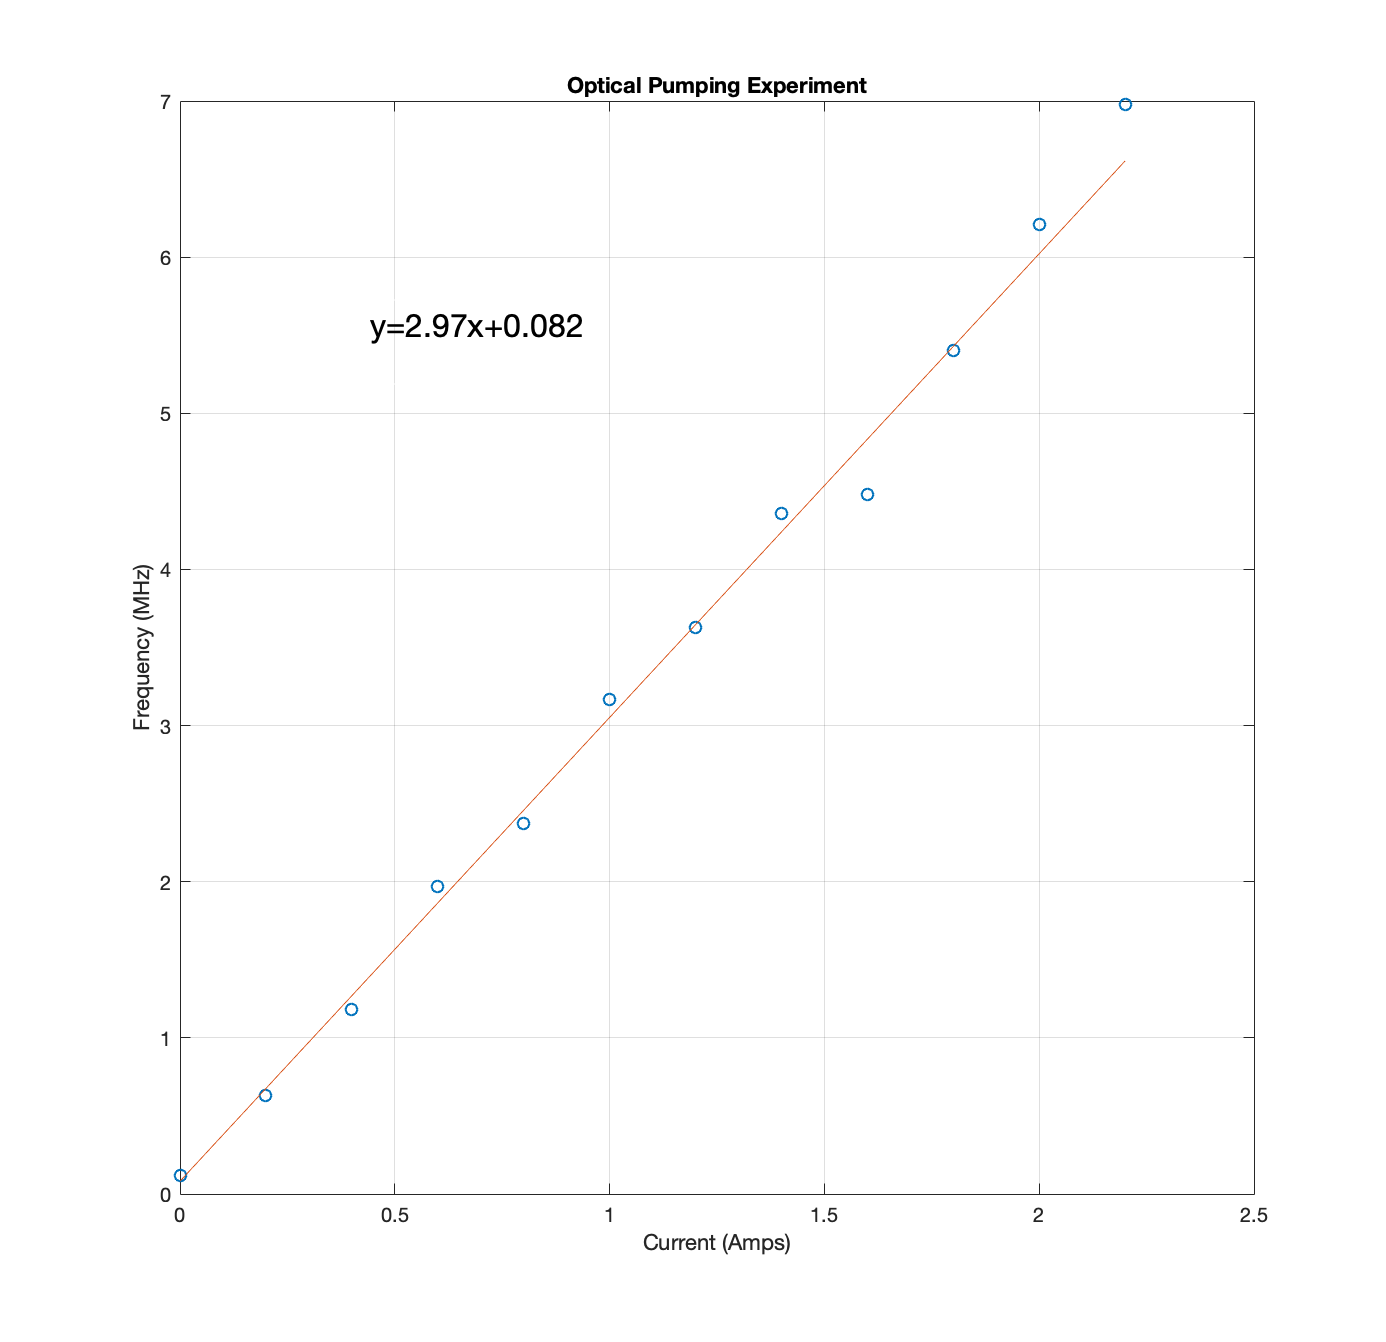
\includegraphics[width=0.8\linewidth]{lateximages/Prob6_4.png}
  \caption{Optical Pumping Experiment with Weighted Least-Squares Fit.}
  \label{fig:boat2}
  \end{figure}
  
  \section*{Problem 7} 

1. Using the propagation of error rules, for a function $x=\log_{10}A$, the error is 

 \[ \sigma_x=\sqrt{\sigma_{xA}^2}=|\frac{\partial x} {\partial A}|\sigma_{A}=\frac{\sigma_{A}}{A*\ln(10)}\]
 
 Now since each $y_i$(A in this case) has a statistical error $\sigma_i$($\sigma_A$ in this case) associated with it, and for simplicity assuming each $\sigma_i$ is the same, we can see that the errors ($\sigma_x$) for a logarithm get smaller (for $x_i>0$) as $y_i$ and $x_i$ gets bigger when plotting a semilog plot of ($x_i$,  $\log_{10}y_i$) when the $y_i$ data points is fitted to an exponential. 
 
 As an example, let's take $y=e^x$, $\sigma_i=10$, and the errors for the semilog plot become $\frac{\sigma_{A}}{A*\ln(10)}=\frac{10}{\ln(10)*e^x}$. On the next page in figure 15 is a semilog plot of $e^x$ with $\sigma_i=10$ associated with each data point. Note how the original error, which was constant for each data point, gets smaller as x gets bigger.
 
 \begin{figure}[H]
  \centering
  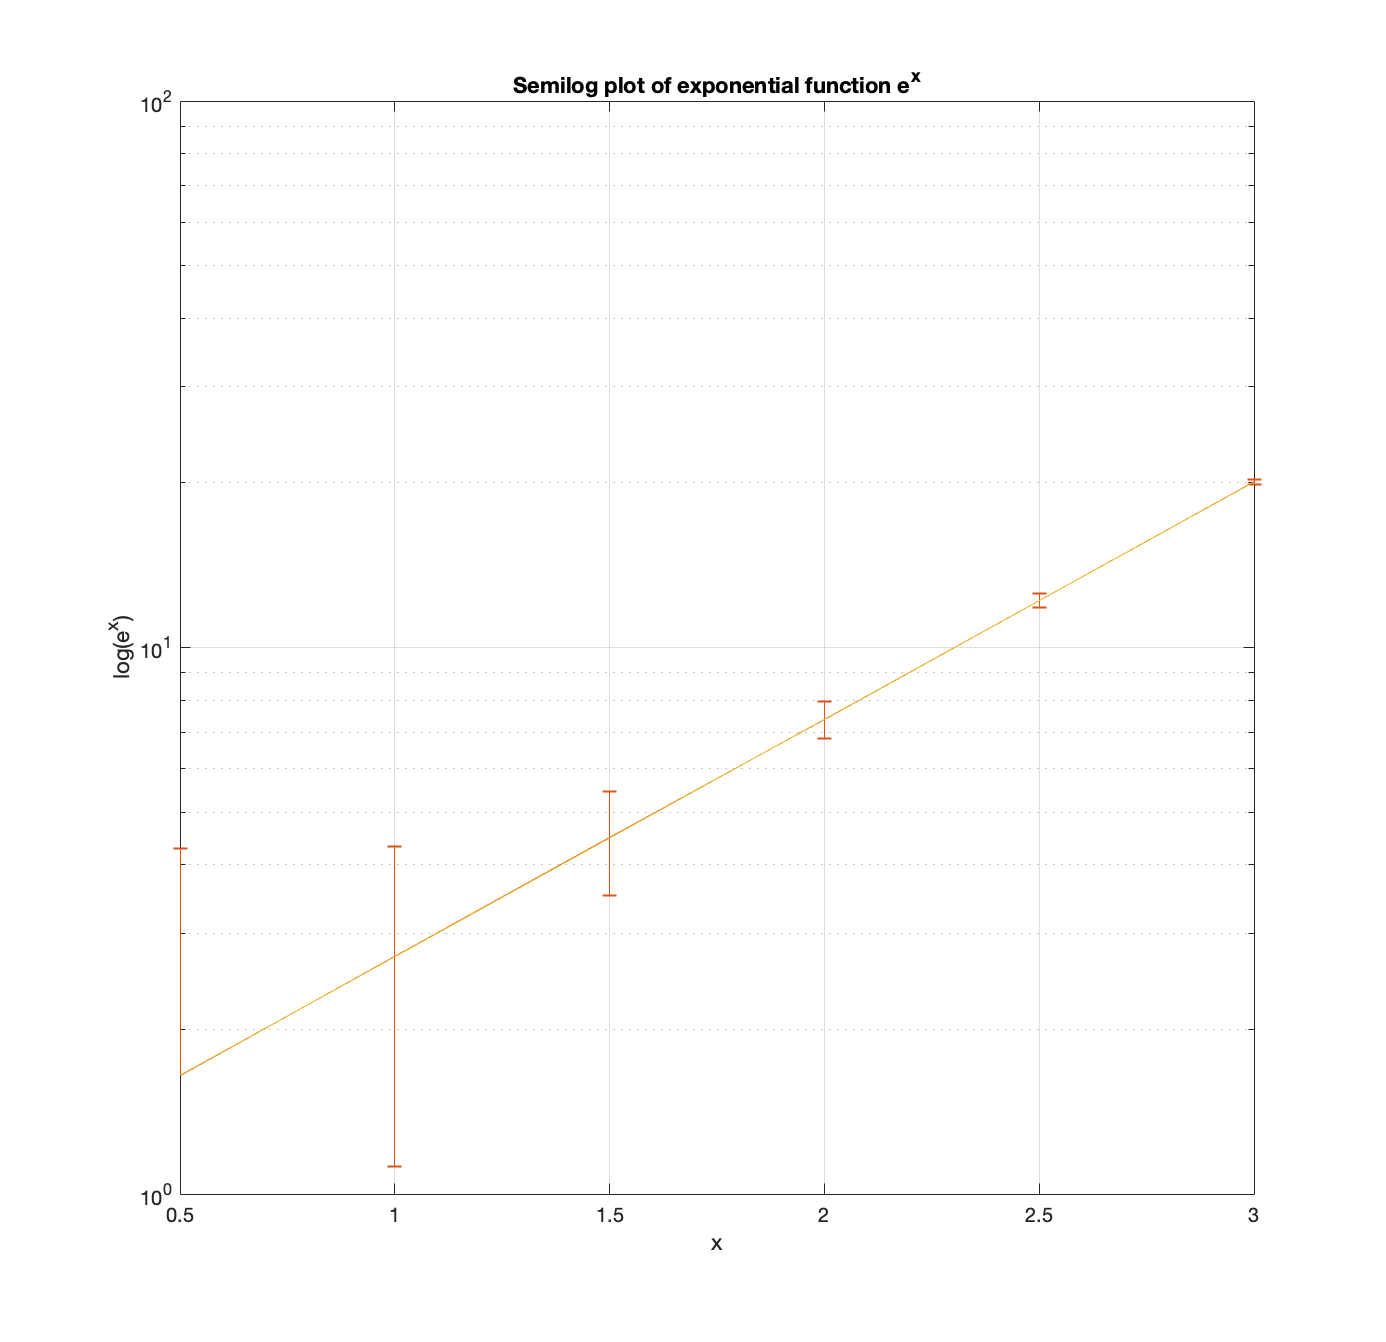
\includegraphics[width=0.8\linewidth]{lateximages/Prob7_1.png}
  \caption{Semilog plot of exponential function.}
  \label{fig:boat2}
  \end{figure}  
 
 \noindent 2. In an experiment we find that $\log_{10}E_0=1.9\pm0.5$. Using the propagation of error rules, for a function $\log_{10}A$, the error is 

 \[ \sigma_x=\sqrt{\sigma_{xA}^2}=|\frac{\partial x} {\partial A}|\sigma_{A}=\frac{\sigma_{A}}{A*\ln(10)}\]
 
 \noindent In this case A is $E_0$ and $\sigma_A$ is the error associated with $E_0$ which I will now refer to as $\sigma_{E_0}$. Now in this case, $\sigma_x=0.5$ and $E_0=10^{1.9}$. So the error associated with $E_0$ is 
 
\[ \sigma_{E_0}=\sigma_{x}*E_0*\ln(10)=\ln(10)*0.5*10^{1.9}=\boxed{91.45}\]

\noindent So we have that $E_0=10^{1.9}\pm91.45$. 

 
 
 
\end{document}